\section{Introduction}
\label{sec:introduction}

\subsection{Background and Motivation}
Time series forecasting lies at the heart of quantitative finance. Hedge funds, asset managers, and proprietary trading desks rely on predictive models to anticipate market movements, optimize portfolio allocation, and manage risk. The ability to forecast financial time series accurately---even marginally---can translate into substantial economic value.

This project addresses the \textbf{Kaggle ``Hedge Fund --- Time Series Forecasting''} competition (competition slug: \texttt{ts-forecasting}), hosted by \emph{A data COMPANY}. The competition ran from January~9, 2026 through April~7, 2026, attracting 3,211 entrants, 1,063 active participants across 982 teams, and 4,127 total submissions. A prize pool of \$10,000 underscored the real-world relevance of the task.

The challenge encapsulates a canonical problem in quantitative research: given a large, anonymized panel of financial time series---each identified by entity codes, sub-categories, and forecast horizons---build models that generalize robustly out-of-sample. The anonymization removes domain shortcuts; success depends entirely on the statistical and machine-learning methodology applied.

\subsection{Problem Statement}
The \textbf{Hedge Fund --- Time Series Forecasting} competition on Kaggle tasks participants with predicting future values of anonymized financial time series. The competition is hosted by \emph{A data COMPANY} and is classified as a \emph{Community Prediction Competition}.

The official description states:
\begin{quote}
\itshape
Participants will receive an integer-indexed time series dataset (\texttt{ts\_index} column), where each record is identified by a code, sub-code, sub-category and forecast horizon. Your objective is to train a model that generalizes robustly out-of-sample and accurately predicts future values for each combination (code, sub-code, sub-category, horizon). Submissions are ranked according to an aggregate out-of-sample metric calculated for all combinations.
\end{quote}

A critical constraint is explicitly stated: \emph{``Your forecast will not use any data whose \texttt{ts\_index} is greater than the \texttt{ts\_index} of the forecast data.''} This enforces strict temporal ordering and prohibits look-ahead bias.

\begin{figure}[H]
\centering
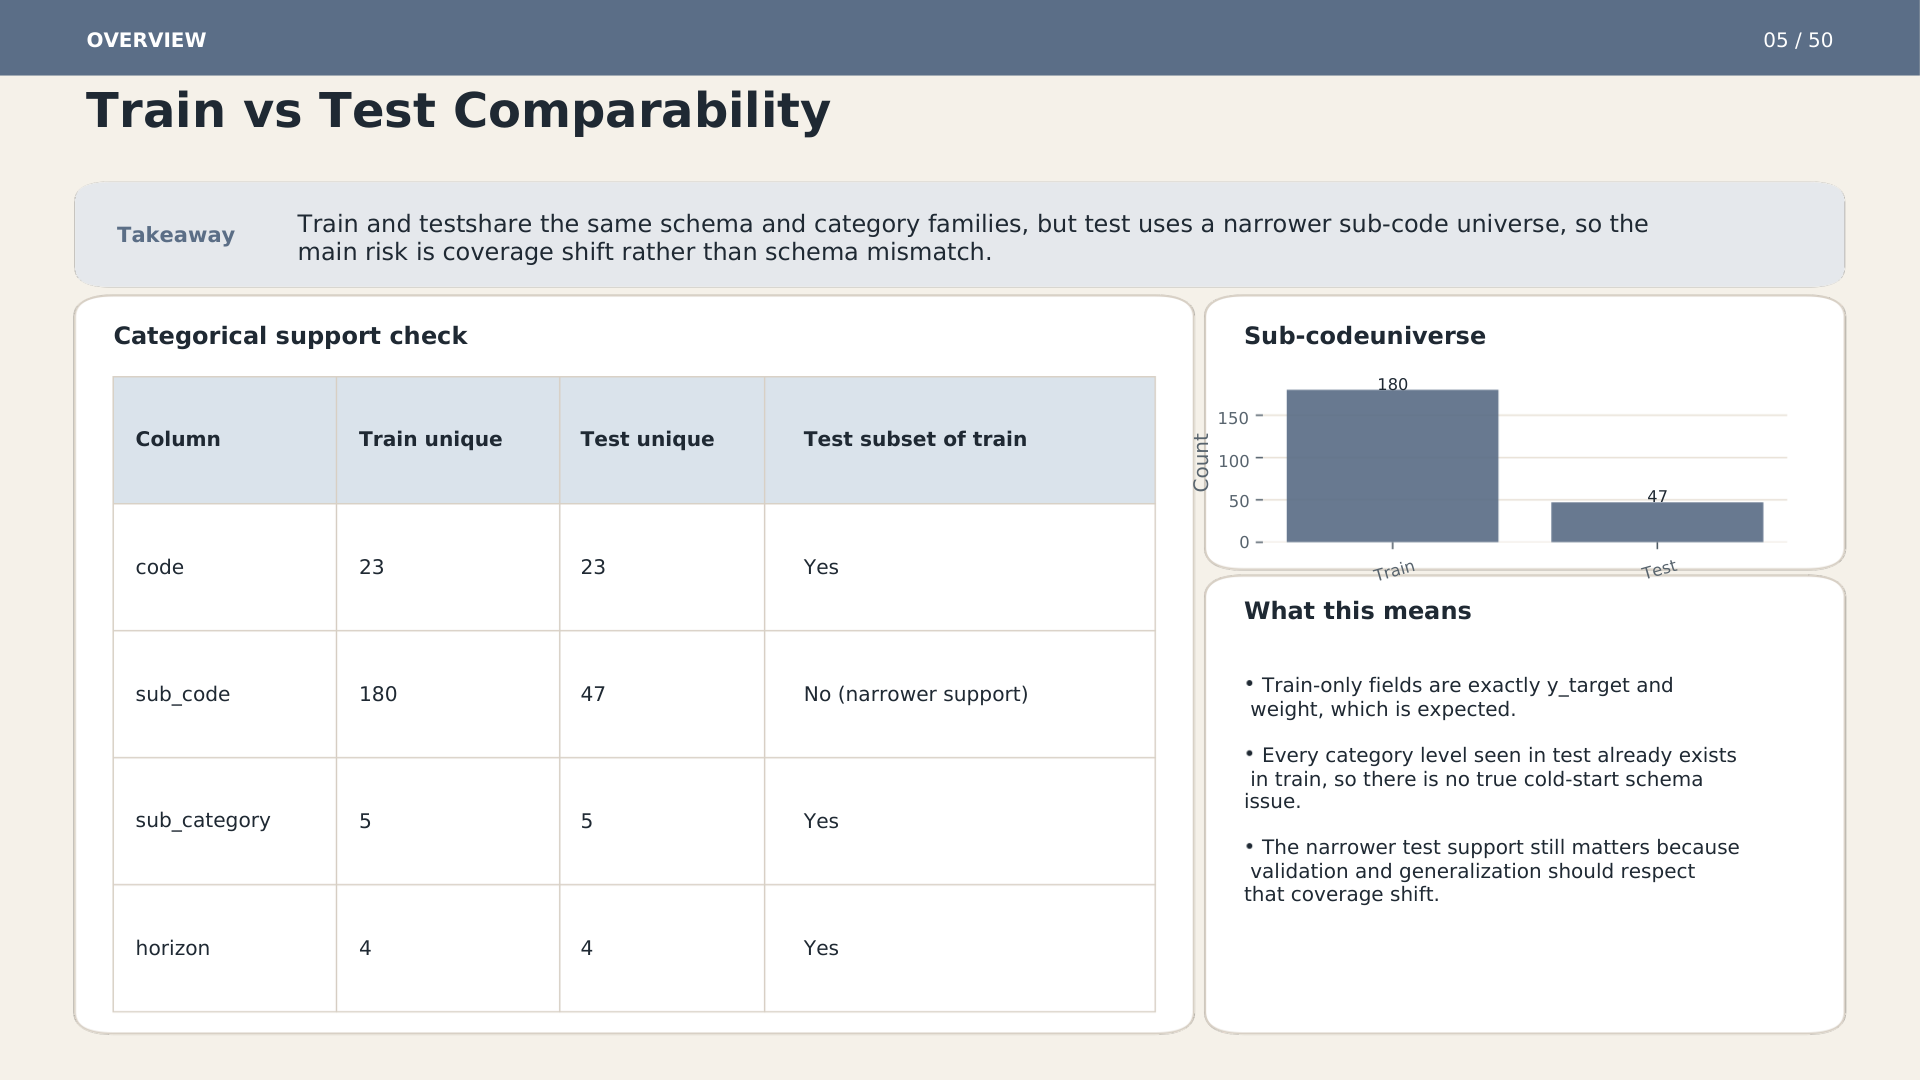
\includegraphics[width=0.95\textwidth]{figures/slide_05.png}
\caption{Train vs.~Test comparability analysis. The categorical support check reveals that train and test share the same schema and category families, but the test set uses a narrower sub-code universe (47 vs.~180), making coverage shift the primary risk.}
\label{fig:train_test_compare}
\end{figure}

\subsection{Objectives}
The objectives of this project are threefold:

\begin{enumerate}[label=(\roman*)]
    \item \textbf{Comprehensive Exploratory Data Analysis (EDA):} Understand the structure, distributional properties, temporal dynamics, and weight distribution of the panel dataset before any modeling.
    \item \textbf{Classical Statistical Modeling:} Establish defensible baselines and univariate benchmarks using AR, MA, ARMA, ARIMA, and SARIMA families, rigorously honoring the stationarity findings from the EDA.
    \item \textbf{Deep Sequence Modeling:} Implement and evaluate recurrent neural network architectures---vanilla RNN, GRU, and LSTM---that can capture nonlinear temporal dependencies the classical models cannot.
\end{enumerate}

